\documentclass[tikz,border=5pt]{standalone}
\usepackage{tikz}

\begin{document}
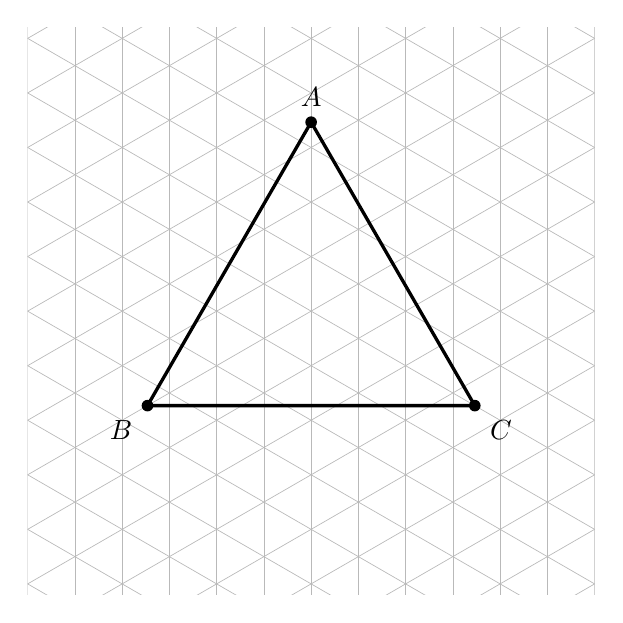
\begin{tikzpicture}[scale=3, line cap=round, line join=round]

  % Styles
  \tikzset{
    grid/.style={line width=0.25pt, gray!55},
    tri/.style={very thick}
  }

  % --- Grid over an open plane (no boundary drawn) ---
  % We clip to a square just to keep the drawing contained; no border is drawn.
  \begin{scope}
    \clip (-1.2,-1.2) rectangle (1.2,1.2);

    % Helper: draw a long straight line with normal angle phi and offset c (n�x = c)
    \pgfmathsetmacro{\L}{3.0} % half-length of drawn line segment (large; clipped by the rectangle)
    \newcommand{\DrawLine}[2]{%
      \pgfmathsetmacro{\phi}{#1}
      \pgfmathsetmacro{\c}{#2}
      \pgfmathsetmacro{\nx}{cos(\phi)} \pgfmathsetmacro{\ny}{sin(\phi)} % unit normal
      \pgfmathsetmacro{\tx}{-sin(\phi)} \pgfmathsetmacro{\ty}{cos(\phi)} % unit tangent
      \pgfmathsetmacro{\cx}{\c*\nx} \pgfmathsetmacro{\cy}{\c*\ny}       % one point on the line
      \draw[grid]
        ({\cx - \L*\tx},{\cy - \L*\ty}) --
        ({\cx + \L*\tx},{\cy + \L*\ty});
    }

    % Triangular grid: three families at 0�, 60�, 120�; evenly spaced
    \pgfmathsetmacro{\d}{0.20} % spacing in normal coordinate
    \foreach \phi in {0,60,120}{
      \foreach \k in {-12,...,12}{
        \pgfmathsetmacro{\c}{\k*\d}
        \DrawLine{\phi}{\c}
      }
    }
  \end{scope}

  % --- Equilateral triangle centered at the origin ---
  \pgfmathsetmacro{\r}{0.80}
  \pgfmathsetmacro{\aA}{ 90}
  \pgfmathsetmacro{\aB}{210}
  \pgfmathsetmacro{\aC}{330}
  \pgfmathsetmacro{\Ax}{\r*cos(\aA)} \pgfmathsetmacro{\Ay}{\r*sin(\aA)}
  \pgfmathsetmacro{\Bx}{\r*cos(\aB)} \pgfmathsetmacro{\By}{\r*sin(\aB)}
  \pgfmathsetmacro{\Cx}{\r*cos(\aC)} \pgfmathsetmacro{\Cy}{\r*sin(\aC)}

  \draw[tri] (\Ax,\Ay) -- (\Bx,\By) -- (\Cx,\Cy) -- cycle;

  % Vertices
  \fill (\Ax,\Ay) circle (0.7pt) node[above=2pt] {$A$};
  \fill (\Bx,\By) circle (0.7pt) node[below left=2pt] {$B$};
  \fill (\Cx,\Cy) circle (0.7pt) node[below right=2pt] {$C$};

\end{tikzpicture}
\end{document}
